\begin{figure}[h!]
	\centering
	
	
	\tikzset{every picture/.style={line width=0.75pt}} %set default line width to 0.75pt        
	
	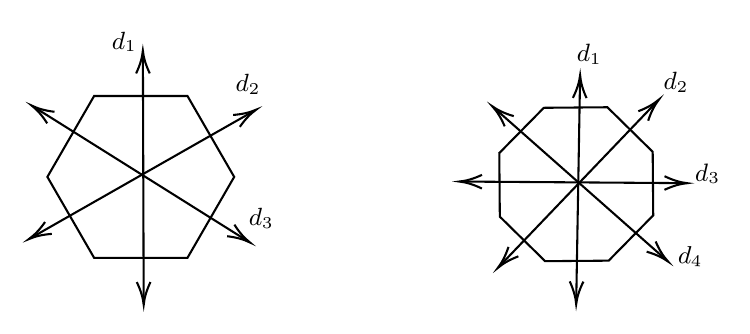
\begin{tikzpicture}[x=0.75pt,y=0.75pt,yscale=-1,xscale=1]
		%uncomment if require: \path (0,300); %set diagram left start at 0, and has height of 300
		
		%Shape: Regular Polygon [id:dp38272018055122115] 
		\draw   (229,100) -- (206.5,138.97) -- (161.5,138.97) -- (139,100) -- (161.5,61.03) -- (206.5,61.03) -- cycle ;
		%Shape: Regular Polygon [id:dp03643618608702448] 
		\draw   (430.63,87.9) -- (430.89,118.52) -- (409.42,140.35) -- (378.81,140.6) -- (356.98,119.14) -- (356.72,88.52) -- (378.19,66.7) -- (408.8,66.44) -- cycle ;
		%Straight Lines [id:da42417542410569764] 
		\draw    (185.39,159.6) -- (185.01,41.2) ;
		\draw [shift={(185,39.2)}, rotate = 89.81] [color={rgb, 255:red, 0; green, 0; blue, 0 }  ][line width=0.75]    (10.93,-3.29) .. controls (6.95,-1.4) and (3.31,-0.3) .. (0,0) .. controls (3.31,0.3) and (6.95,1.4) .. (10.93,3.29)   ;
		\draw [shift={(185.4,161.6)}, rotate = 269.81] [color={rgb, 255:red, 0; green, 0; blue, 0 }  ][line width=0.75]    (10.93,-3.29) .. controls (6.95,-1.4) and (3.31,-0.3) .. (0,0) .. controls (3.31,0.3) and (6.95,1.4) .. (10.93,3.29)   ;
		%Straight Lines [id:da8675028417491909] 
		\draw    (131.74,129.01) -- (237.86,68.59) ;
		\draw [shift={(239.6,67.6)}, rotate = 150.35] [color={rgb, 255:red, 0; green, 0; blue, 0 }  ][line width=0.75]    (10.93,-3.29) .. controls (6.95,-1.4) and (3.31,-0.3) .. (0,0) .. controls (3.31,0.3) and (6.95,1.4) .. (10.93,3.29)   ;
		\draw [shift={(130,130)}, rotate = 330.35] [color={rgb, 255:red, 0; green, 0; blue, 0 }  ][line width=0.75]    (10.93,-3.29) .. controls (6.95,-1.4) and (3.31,-0.3) .. (0,0) .. controls (3.31,0.3) and (6.95,1.4) .. (10.93,3.29)   ;
		%Straight Lines [id:da30906746309807165] 
		\draw    (133.09,66.66) -- (234.91,130.54) ;
		\draw [shift={(236.6,131.6)}, rotate = 212.1] [color={rgb, 255:red, 0; green, 0; blue, 0 }  ][line width=0.75]    (10.93,-3.29) .. controls (6.95,-1.4) and (3.31,-0.3) .. (0,0) .. controls (3.31,0.3) and (6.95,1.4) .. (10.93,3.29)   ;
		\draw [shift={(131.4,65.6)}, rotate = 32.1] [color={rgb, 255:red, 0; green, 0; blue, 0 }  ][line width=0.75]    (10.93,-3.29) .. controls (6.95,-1.4) and (3.31,-0.3) .. (0,0) .. controls (3.31,0.3) and (6.95,1.4) .. (10.93,3.29)   ;
		%Straight Lines [id:da65453798610991] 
		\draw    (393.8,159.32) -- (395.63,53.03) ;
		\draw [shift={(395.66,51.03)}, rotate = 90.98] [color={rgb, 255:red, 0; green, 0; blue, 0 }  ][line width=0.75]    (10.93,-3.29) .. controls (6.95,-1.4) and (3.31,-0.3) .. (0,0) .. controls (3.31,0.3) and (6.95,1.4) .. (10.93,3.29)   ;
		\draw [shift={(393.77,161.32)}, rotate = 270.98] [color={rgb, 255:red, 0; green, 0; blue, 0 }  ][line width=0.75]    (10.93,-3.29) .. controls (6.95,-1.4) and (3.31,-0.3) .. (0,0) .. controls (3.31,0.3) and (6.95,1.4) .. (10.93,3.29)   ;
		%Straight Lines [id:da5174940913781368] 
		\draw    (357.35,142.45) -- (432.26,64.18) ;
		\draw [shift={(433.64,62.73)}, rotate = 133.74] [color={rgb, 255:red, 0; green, 0; blue, 0 }  ][line width=0.75]    (10.93,-3.29) .. controls (6.95,-1.4) and (3.31,-0.3) .. (0,0) .. controls (3.31,0.3) and (6.95,1.4) .. (10.93,3.29)   ;
		\draw [shift={(355.97,143.9)}, rotate = 313.74] [color={rgb, 255:red, 0; green, 0; blue, 0 }  ][line width=0.75]    (10.93,-3.29) .. controls (6.95,-1.4) and (3.31,-0.3) .. (0,0) .. controls (3.31,0.3) and (6.95,1.4) .. (10.93,3.29)   ;
		%Straight Lines [id:da7207208027265464] 
		\draw    (339.43,102.24) -- (445.25,103) ;
		\draw [shift={(447.25,103.02)}, rotate = 180.41] [color={rgb, 255:red, 0; green, 0; blue, 0 }  ][line width=0.75]    (10.93,-3.29) .. controls (6.95,-1.4) and (3.31,-0.3) .. (0,0) .. controls (3.31,0.3) and (6.95,1.4) .. (10.93,3.29)   ;
		\draw [shift={(337.43,102.23)}, rotate = 0.41] [color={rgb, 255:red, 0; green, 0; blue, 0 }  ][line width=0.75]    (10.93,-3.29) .. controls (6.95,-1.4) and (3.31,-0.3) .. (0,0) .. controls (3.31,0.3) and (6.95,1.4) .. (10.93,3.29)   ;
		%Straight Lines [id:da7287534383817258] 
		\draw    (354.82,67.27) -- (436.57,139.47) ;
		\draw [shift={(438.07,140.8)}, rotate = 221.45] [color={rgb, 255:red, 0; green, 0; blue, 0 }  ][line width=0.75]    (10.93,-3.29) .. controls (6.95,-1.4) and (3.31,-0.3) .. (0,0) .. controls (3.31,0.3) and (6.95,1.4) .. (10.93,3.29)   ;
		\draw [shift={(353.32,65.94)}, rotate = 41.45] [color={rgb, 255:red, 0; green, 0; blue, 0 }  ][line width=0.75]    (10.93,-3.29) .. controls (6.95,-1.4) and (3.31,-0.3) .. (0,0) .. controls (3.31,0.3) and (6.95,1.4) .. (10.93,3.29)   ;
		
		% Text Node
		\draw (168.6,28.6) node [anchor=north west][inner sep=0.75pt]  [font=\small]  {$d_{1}$};
		% Text Node
		\draw (228.2,49) node [anchor=north west][inner sep=0.75pt]  [font=\small]  {$d_{2}$};
		% Text Node
		\draw (234.6,113.6) node [anchor=north west][inner sep=0.75pt]  [font=\small]  {$d_{3}$};
		% Text Node
		\draw (441.48,131.94) node [anchor=north west][inner sep=0.75pt]  [font=\small,rotate=-1.57]  {$d_{4}$};
		% Text Node
		\draw (392.55,34.66) node [anchor=north west][inner sep=0.75pt]  [font=\small,rotate=-359.55]  {$d_{1}$};
		% Text Node
		\draw (434.39,48.18) node [anchor=north west][inner sep=0.75pt]  [font=\small,rotate=-359.8]  {$d_{2}$};
		% Text Node
		\draw (449.46,92.26) node [anchor=north west][inner sep=0.75pt]  [font=\small,rotate=-359.03]  {$d_{3}$};
		
		
	\end{tikzpicture}
\end{figure}